\section{Liyana Majdah Rahma}
{\Large \textbf{Pemahaman Teori}}
\subsection{Soal No. 1}
Apa itu fungsi device manager di windows dan folder /dev di linux?

\hfill \break
Device Manager  dapat  membantu dalam mengelola  semua hardware yang terpasang  dalam suatu sistem Windows. 
 Berikut fungsi kegunaan Device Manager antara lain adalah :
\begin{enumerate}
	\item Menunjukkan status suatu hardware.
	\item Menunjukkan informasi detil suatu hardware.
	\item Mengelola driver hardware
	\item Disable dan Enable hardware
	\item Mengidentifikasi konflik antar perangkat keras.
\end{enumerate}

\hfill \break
Folder /bin merupakan isi program binner yang harus ada apabila sistem yang dipasang dalam mode single-user, dan juga  ada beberapa program penting seperti bash.

\subsection{Soal No. 2}
Jelaskan langkah-langkah instalasi driver dari arduino!

\hfill \break
Berikut ini adalah langkah-langkah instalasi driver dari Arduino UNO di Windows:

\begin{enumerate}
	\item Langkah pertama Hubungkan sistem minimun Arduino Uno ke komputer dengan kabel USB .
	\item Lalu pada bagian kanan didesktop PC , akan muncul popup “Installing device driver software” seperti pada gambar dibawah ini.
	\item Kemudian jika sistem  operasi Windows tidak menyediakan driver untuk Arduino Uno,maka harus  melakukan instalasinya harus dilakukan secara manual.
	\item Lalu  Buka Device Manager,  dengan cara pada bagian Search Program and Files lalu ketikkan “device manager” (tanpa tanda petik). 
	\item kemudian Pada bagian COntrol Panel akan muncul Device Manager, lalu klik untuk menjalankan program tersebut.
	\item Setelah itu cari  Unknown device pada bagian Other device, biasanya terdapat tanda seru berwarna kuning, itu disebabkan karena penginstallan gagal.
	\item Klik kanan pada bagian  “Unknown device” kemudian pilih Update Driver Software.
	\item kemudian cari Browse my computer for driver software pada laptop anda.
	\item setelah itu lakukan dengan mengklik Install pada tampilan Windows Security.
	\item Jika instalasi driver pada laptop anda berhasil maka akan muncul Windows has successfully updated your driver software.
	\item Perhatikan dan ingat nama COM Arduino Uno, karena nama COM ini yang akan digunakan untuk meng-upload program nantinya
\end{enumerate}

\subsection{Soal No. 3}
Jelaskan bagaimana cara membaca baudrate dan port dari komputer yang sudah terinstall driver!

\hfill \break
\textbf{Membaca Port dari Komputer}

\begin{enumerate}
	\item Hubungkan modul TX-RX serial dengan komputer melalui serial port menggunakan DB9 cable extension.
	\item Buka Hyper Terminal dengan menekan start kemudian All progams lalu Accessories kemudian Communications lalu Hyper Terminal.
	\item Ketik nama untuk Connection Description, misal coba, kemudian tekan OK.
	\item Pada Connect to, pilihlah COM port yang dipakai di Connect using, kemudian tekan OK.
	\item Masukkan nilai-nilai port settingnya, sesuai dengan DCE-nya. Kemudian tekan OK.
\end{enumerate}



\subsection{Soal No. 4}
Jelaskan sejarah library pyserial!.

\hfill \break
PySerial adalah library/modul Python siap-pakai dan gratis yang dibuat untuk memudahkan kita dalam membuat program komunikasi data serial RS232 dalam bahasa Python.

\subsection{Soal No. 5}
Jelaskan fungsi-fungsi apa saja yang dipakai dari library pyserial!

\hfill \break
Fungsi-fungsi yang dipakai dari library PySerial, yaitu:
\begin{enumerate}
	\item Serial - fungsi ini untuk membuka port serial.
	\item write(data) - fungsi ini menulis data lewat port serial.
	\item readline() - fungsi ini membaca sebuah string dari port serial.
	\item read(size) - fungsi ini untuk membaca jumlah byte dari port serial.
	\item close() - fungsi ini untuk menutup port serial.
\end{enumerate}

\subsection{Soal No. 6}
Jelaskan kenapa butuh perulangan dan tidak butuh perulangan dalam membaca serial!

\hfill \break
Pada saat membaca serial di Arduino diperlukan perulangan agar dapat membaca data secara berulang kali sehingga data yang muncul banyak. Sedangkan apabila tidak membutuhkan perulangan maka Arduino hanya akan membaca data sekali saja.

\subsection{Soal No. 7}
Jelaskan bagaimana cara membuat fungsi yang mengunakan pyserial!

\hfill \break
Fungsi yang berada pada Python, dibuat dengan nama kata kunci def kemudian diikuti dengan nama fungsinya pada pyhton.
Seperti halnya dengan blok kode yang lain, kita juga harus memberikan identasi untuk menuliskan isi fungsi.

\section{Rangga Putra Ramdhani}
\subsection{ Apa itu fungsi device manager di windows dan folder /dev di linux}
Device Manager adalah Panel Kontrol dalam sistem operasi Microsoft Windows. Ini memungkinkan pengguna untuk melihat dan mengontrol perangkat keras yang terpasang pada komputer. Ketika beberapa bagian perangkat keras tidak berfungsi, perangkat keras yang terkait akan disorot oleh pengguna. Daftar perangkat keras dapat disortir berdasarkan berbagai kriteria.
Untuk setiap perangkat, pengguna dapat:
\begin{itemize}
     \item Menyediakan driver perangkat sesuai dengan Model Driver Windows
     \item Aktifkan atau nonaktifkan perangkat
     \item Beri tahu Windows untuk mengabaikan perangkat yang tidak berfungsi
     \item Lihat sifat teknis lainnya
\end{itemize}
Device Manager diperkenalkan dengan Windows 95 dan kemudian ditambahkan ke Windows 2000. Dalam versi berbasis NT, ini dimasukkan sebagai snap-in Konsol Manajemen Microsoft.\newline

/ dev adalah lokasi file khusus atau perangkat. Ini adalah direktori yang sangat menarik yang menyoroti satu aspek penting dari sistem file Linux - semuanya adalah file atau direktori.


\subsection{Jelaskan langkah-langkah instalasi driver dari Arduino}
Berikut ini merupakan langkah-langkah untuk melakukan instalasi driver Arduino
\begin{itemize}
	\item Pertama-tama, pasang board arduino pada pc. Kemudian tunggu sampai windows mencoba menginstal sendiri. jika gagal, lanjutkan ke step selanjutnya
	\item buka Device Manager 
	\item Cari nama arduino atau "Unknown Device"
	\item klik kanan pada unknown device , dan pilih update software
	\item Cari folder instalan software arduino
	\item klik Next
	\item Jika telah berhasil, maka proses instal driver sudah selesai
\end{itemize}

\subsection{Jelaskan bagaimana cara membaca baudrate dan port dari komputer yang sudah terinstal driver}
Berikut ini merupakan cara membaca baudrate dan port dari komputer yang sudah terinstal driver :
\begin{itemize}
	\item Sambungkan port USB arduino dengan port USB pc
	\item Kemudian buka software arduino pada pc
	\item Setelah itu, pilih tipe arduino yang digunakan
	\item Kemudian memilih serial port yang aktif  
	\item Selanjutnya untuk memasukkan program pada arduino, klik tombol upload
	\item Setelah proses upload selesai, buka fitur serial monitor
	\item Lalu sesuaikan Baudrate pada serial monitor dengan Baudrate yang terdapat pada program
\end{itemize}

\subsection{Jelaskan sejarah library pyserial}
Pyserial berguna untuk merangkum akses untuk port serial. Pyserial menyediakan backends untuk Python yang berjalan di Windows, Linux, BSD (mungkin sistem yang mendukung POSIX), Jython dan IronPython (.NET dan Mono). Modul bernama "serial" secara otomatis memilih backend yang sesuai. Antarmuka berbasis kelas yang sama pada semua platform yang didukung.
Akses ke pengaturan port melalui properti Python.
Dukungan untuk berbagai ukuran byte, bit stop, paritas dan kontrol aliran dengan RTS / CTS dan / atau Xon / Xoff.
Bekerja dengan atau tanpa menerima batas waktu.
File seperti API dengan "read" dan "write" ("readline" dll. Juga didukung).
File-file dalam paket ini adalah 100 persen Python murni.
Port diatur untuk transmisi biner. Tidak ada stripping byte NULL, terjemahan CR-LF dll. (Yang berkali-kali diaktifkan untuk POSIX.) Ini membuat modul ini bermanfaat secara universal.
Kompatibel dengan pustaka io (Python 2.6+)

\subsection{Jelaskan fungsi-fungsi apa saja yang dipakai dari library pyserial}
Serial – fungsi ini untuk membuka port serial
Write(data) – untuk menulis data lewat port serial
Readline() – untuk membaca string dari port serial
Read(size) – untuk membaca jumlah byte dari port serial
Close() – ini untuk menutup port serial 

\subsection{Jelaskan kenapa butuh perulangan dalam tidak butuh perulangan dalam membaca serial}
Perualangan dalam bahasa pemrograman berfungsi menyuruh komputer melakukan sesuatu secara berulang-ulang. Terdapat dua jenis perualangan dalam bahasa pemrograman python, yaitu perulangan dengan for dan while.
Perulangan for disebut counted loop (perulangan yang terhitung), sementara perulangan while disebut uncounted loop (perulangan yang tak terhitung). Perbedaan yang terlihat adalah pada perulangan for digunakan untuk mengulangi kode yang sudah diketahui banyak perulangannya. Sedangkan perulangan while digunakan pada perulangan yang memiliki syarat dan tidak tentu berapa banyak perulangannya.
Perulangan diperlukan agar dapat membaca data secara berulang kali sehingga data yang muncul lebih dari satu.  Sedangkan apabila tidak memakai perulangan maka data akan terbaca satu kali saja.

\subsection{Jelaskan bagaimana cara membuat fungsi yang mengunakan pyserial}
Fungsi yang berada pada Python, dibuat dengan nama kata kunci def kemudian diikuti dengan nama fungsinya pada pyhton.
Seperti halnya dengan blok kode yang lain, kita juga harus memberikan identasi untuk menuliskan isi fungsi.

\subsection{Plagiarisme}
\begin{figure}[h]
\centering
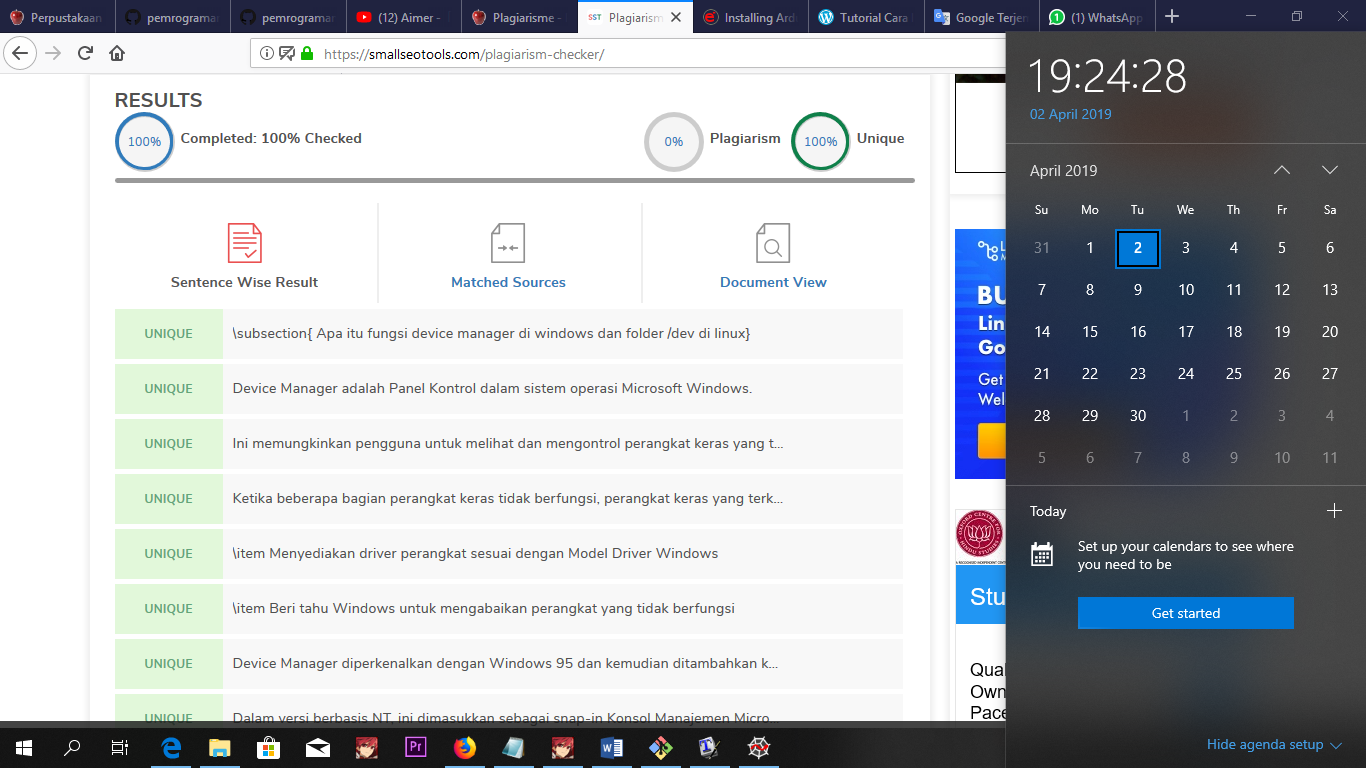
\includegraphics[scale=0.2]{figures/5/Teori/1174056/plagiat.png}
\caption{Plagiarisme}
\label{fig:plagiat}
\end{figure}